\chapter{The Protocol}\label{ch:protocol}

In this chapter, we present our privacy-preserving monitoring protocol. We begin by restating the monitoring problem in the language of reactive two-party computation (\cref{sec:framework}), then briefly discuss the design space (\cref{sec:designspace}). The protocol itself is developed in two steps: first for the setting where the specification circuit is known to both parties (\cref{sec:openstep}), and then for the setting where the circuit must also be kept secret from the System (\cref{sec:hiddenstep}).

\section{Reactive monitoring as secure computation}\label{sec:framework}

Monitoring differs from textbook secure computation in one important way: it is \emph{stateful}. The System and the Monitor do not evaluate a function once; they evaluate it \emph{every round}, and each evaluation depends on state produced by the previous one. A protocol that achieves this is what we call a \emph{reactive secure monitoring protocol}.

Concretely, recall from \cref{ch:formulation} that the monitoring functionality is determined by a circuit~$\Cc$ (encoding both the flag function~$\isbad$ and the state-update function~$\mupdate$), an initial monitor state~$\mu[1]$, and a stream of System inputs $\sigma[1],\sigma[2],\ldots$ At every round~$r$ the functionality produces the verdict $\tau[r] = \isbad(\sigma[r],\mu[r])$ and internally advances its state to $\mu[r+1] = \mupdate(\sigma[r],\mu[r])$. Neither party ever sees the intermediate states.

A protocol~$\pi$ \emph{securely realizes} this functionality if it satisfies four properties:

\begin{enumerate}
    \item \textbf{Correctness.} In every round the Monitor obtains the same verdict $\tau[r] = \isbad(\sigma[r],\mu[r])$ it would have received from the ideal-world TTP, with overwhelming probability (see \cref{def:correctness}).
    \item \textbf{System privacy.} A simulator $\Sc_\Mc$, given only the Monitor's own inputs $(\Cc,\mu[1])$ and the verdicts $\tau[1],\ldots,\tau[\ell]$, can produce a transcript indistinguishable from the Monitor's real view. The Monitor learns nothing about $\sigma[r]$ beyond what the verdict implies.
    \item \textbf{Monitor privacy.} A simulator $\Sc_\Pc$, given only the System's inputs and (in the open-specification setting) the circuit~$\Cc$, can produce a transcript indistinguishable from the System's real view. The System learns nothing about $\mu[r]$ for any~$r$.
    \item \textbf{Specification privacy (hidden-specification setting only).} The System's simulator needs only the circuit \emph{size}~$c$, not $\Cc$ itself. This hides the circuit topology---and hence the specification---from the System.
\end{enumerate}

\noindent After an initial setup phase, each subsequent round consists of one message from the System to the Monitor, plus a single-bit response (\proceed{} or \terminate{}).  As noted in \cref{sec:monitoringprotocol}, this ``single message'' is largely a bookkeeping convenience: in the hidden-specification step every wire label is a group element produced by bare modular exponentiation, with no batching or compression, so a single round's payload can run to tens of megabytes (see \cref{fig:locks_message_P2}).  Many MPC protocols get by with $O(\text{depth}(\Cc))$ or $O(\log c)$ rounds of interaction, which would be perfectly acceptable here; we impose the single-message constraint because it simplifies the security argument and because, at the scale of our experiments, the bottleneck is computation (the modular exponentiations themselves) rather than the number of network round-trips.

Our protocol provides two instantiations with increasing privacy:

\begin{enumerate}
    \item \textbf{Open-specification step} (\cref{sec:openstep}). Both parties know~$\Cc$. The key idea is a reactive adaptation of Yao's garbled circuits in which wire labels for the monitor state are reused across rounds to maintain state without revealing it.
    \item \textbf{Hidden-specification step} (\cref{sec:hiddenstep}). Only the Monitor knows~$\Cc$; the System knows only the gate count~$c$. The additional tool is DDH-based topology hiding, following~\cite{LWY22}.
\end{enumerate}

\section{Design space}\label{sec:designspace}

Before describing the protocol, we briefly justify the three main design choices.

\paragraph{Garbled circuits over FHE and secret sharing.}
As discussed in \cref{ch:related}, the FHE-based protocols of Banno et al.~\cite{BMMBWS22} and Waga et al.~\cite{WMSMBBS24} operate in a different trust model, and their evaluation cost is linear in the DFA size of the specification---exponentially larger than the circuit representation for specifications with large state spaces (see \cref{table:compareBanno}). Secret-sharing-based MPC requires three or more parties~\cite{GMW87} and does not directly apply to our two-party setting. Two-party protocols for reactive functionalities are standard~\cite{HL10}, but typically require multiple message exchanges per round (at least three for OT-based constructions~\cite{CSW20}). Garbled circuits give us a single-message-per-round design after the initial setup, with the Monitor evaluating non-interactively.

\paragraph{Reactive label reuse.}
A naïve approach would run an independent Yao instance per round. That forces oblivious transfer (OT) in every round (at least three messages) and requires explicitly transferring the monitor state---either in the clear (breaking privacy) or via further OT. Our protocol avoids both problems by \emph{reusing labels}: the wire labels assigned to the monitor-state output wires of round~$r$ become the input labels for round~$r{+}1$. The Monitor already holds the correct labels from evaluating the previous round, so no OT is needed after round~1, and it never learns the actual bit values of~$\mu[r]$. The security of this reuse relies on a hybrid argument detailed in \cref{app:proofs}.

\paragraph{DDH-based topology hiding.}
In the hidden-specification setting, the circuit topology must be concealed. Universal circuits~\cite{Val76} would impose a $\Theta(\log^2 c)$ blowup in circuit size. Homomorphic-encryption-based PFE~\cite{KM11} requires multi-round interaction during setup. The DDH-based approach of Liu et al.~\cite{LWY22} avoids both: the Monitor assigns random group elements as \emph{base labels} to feed-out wires and exponentiates them to produce feed-in labels; by the DDH assumption (\cref{lemma:DDHprop}), the System cannot tell which feed-out wire connects to which feed-in wire. Base labels are set once during setup and reused across all rounds, amortizing the cost. Our extension beyond~\cite{LWY22} adds reactive state: exponents from round~$r$ carry over to round~$r{+}1$, enabling stateful computation while preserving topology hiding.

\section{Circuit conventions and notation}\label{sec:conventions}

Every specification is compiled into a Boolean circuit~$\Cc$ before the protocol begins. We fix the following conventions.

\begin{itemize}
    \item \textit{Size.} The circuit contains $c$~gates, $s{+}m$ input wires (the first~$m$ for the Monitor's state, the remaining~$s$ for the System's data), and $m{+}1$ output wires (the first~$m$ feeding back the updated state, the last carrying the verdict bit~$\tau[r]$).
    \item \textit{Gates.} Every gate is a NAND gate with exactly two \emph{feed-in} wires (left and right) and one \emph{feed-out} wire. We write $G_1,\ldots,G_c$ for the gates; gate~$G_j$ has feed-in wires $\iota_{2j-1}$ (left) and $\iota_{2j}$ (right), and feed-out wire $\omega_{m+s+j}$.
    \item \textit{Wires.} A \emph{feed-out} wire exits a gate (or serves as a circuit input); a \emph{feed-in} wire enters a gate. Every feed-in wire is connected to exactly one feed-out wire, but a feed-out wire may fan out to several feed-in wires. There are $I = 2c$ feed-in wires and $c{+}s{+}m$ feed-out wires. The first $m{+}s$ feed-out wires $\omega_1,\ldots,\omega_{m+s}$ are the circuit inputs; among these, $\omega_1,\ldots,\omega_m$ carry the Monitor's state and $\omega_{m+1},\ldots,\omega_{m+s}$ carry the System's data. The $O = c{+}s{-}1$ non-output feed-out wires plus the $m{+}1$ output wires fill out the rest: the output wires are $\omega_{O+1},\ldots,\omega_{O+m}$ (feedback state) and $\omega_{O+m+1}$ (the $\isbad$ bit).
    \item \textit{Fan-out restriction.} We assume that output wires of the circuit do not connect back to any feed-in wires.
\end{itemize}

\noindent See the black labels in \cref{fig:exponentsingoingwires} for a pictorial summary.

\section{Step~1: Monitoring with an open specification}\label{sec:openstep}

We begin with the conceptually simpler case: both parties already know the specification circuit~$\Cc$. The internal state computed by the circuit is still kept secret. The protocol is a reactive adaptation of Yao's garbled circuits (see \cref{sec:yao}); the central idea is that wire labels for the monitor state are reused from one round to the next, avoiding additional oblivious transfer after the first round.

\paragraph{Setup (round~0).}\label{protocol1}
Both parties agree on the circuit~$\Cc$ and a security parameter~$n$. The Monitor holds an $m$-bit initial state $\mu[1]$. The System and Monitor execute a $1$-out-of-$2$ oblivious transfer for each of the $m$ state bits: the System acts as sender with random label pairs $(w_i^0[1],w_i^1[1])$, and the Monitor acts as chooser with choice bit~$\mu_i[1]$. At the end of this step, the Monitor holds the labels $w_i^{\mu_i[1]}[1]$ for $i \in \{1,\ldots,m\}$ without the System learning $\mu[1]$, and without the Monitor learning the other labels.

\paragraph{Round~$r$ ($r \geq 1$).}
The System holds the current data item $\sigma[r] \in \{0,1\}^s$. It proceeds as follows.

\begin{enumerate}
    \item \textbf{Generate feed-out labels.} For every feed-out wire $\omega_i$ with $i \in \{m{+}1,\ldots,c{+}s{+}m\}$, the System draws two fresh random strings $w_i^0[r]$ and $w_i^1[r]$.
    \item \textbf{Reuse state labels.} For the Monitor-state input wires $\omega_1,\ldots,\omega_m$:
        \begin{itemize}
            \item In round~$1$, the labels $w_i^0[1], w_i^1[1]$ were already generated during setup.
            \item In rounds $r > 1$, the System reuses the labels of the feedback wires from the previous round: $w_i^b[r] \gets w_{O+i}^b[r{-}1]$ for $b \in \{0,1\}$ and $i \in \{1,\ldots,m\}$.
        \end{itemize}
    \item \textbf{Assign feed-in labels.} Each feed-in wire $\iota_i$ inherits the labels of the feed-out wire it is connected to: if $\omega_j$ connects to~$\iota_i$, then $u_i^b[r] = w_j^b[r]$.
    \item \textbf{Garble and send.} For each gate $G_j$, the System computes the garbled gate
    \[
      \encGG_j[r] = \encYao_{G_j} \begin{pmatrix}
         \left[u_{2j-1}^0[r], u_{2j-1}^1[r]\right], \\
         \left[u_{2j}^0[r], u_{2j}^1[r]\right], \\
         \left[w_{m+s+j}^0[r],   w_{m+s+j}^1[r]\right]
      \end{pmatrix}
    \]
    and sends to the Monitor: all garbled gates $\encGG_j[r]$, the System's input labels $w_{m+i}^{\sigma_i[r]}[r]$ for $i \in \{1,\ldots,s\}$, and both flag labels $w_{O+m+1}^0[r]$, $w_{O+m+1}^1[r]$.
    \item \textbf{Evaluate.} The Monitor ungarbles the circuit bottom-up using the monitor-state labels it already holds (from setup or the previous round) together with the System's input labels. After evaluation, the Monitor holds one label per output wire: the state-feedback labels $w_{O+i}^{\mu_i[r+1]}[r]$ (which become the input labels for round~$r{+}1$) and the flag label, which it compares against the two flag labels to determine~$\tau[r]$.
\end{enumerate}

The following theorem shows that the open-specification step is correct and secure, assuming that the encryption is secure under the chosen plaintext attack (CPA)~\cite{Bir11}.

\begin{restatable}{theorem}{Protocolonesecure}\label{thm:Protocol1secure}
    Under CPA-secure encryption and semi-honest oblivious transfer, the open-specification step is a correct and secure monitoring protocol (without specification hiding) for any polynomial number of rounds.
\end{restatable}


\section{Step~2: Extending to hidden specifications}\label{sec:hiddenstep}

% Labelling figures
\begin{figure}[t]
\centering
    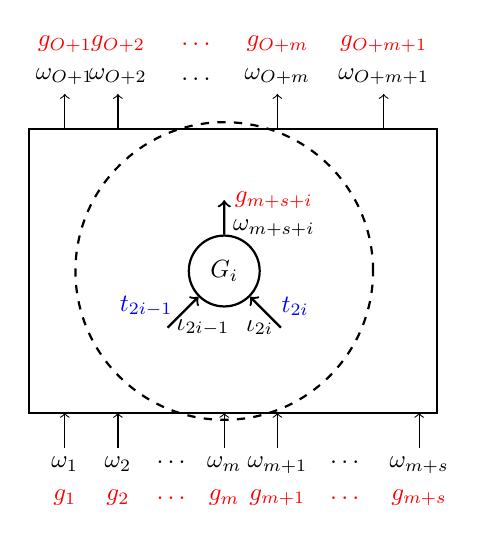
\begin{tikzpicture}[scale = 0.9, transform shape]
        \draw[thick] (0.25,0) rectangle (6,4);
        
        \node[circle, draw, thick, minimum size=1cm] (A) at (3, 2) {$G_i$};
            
        \draw[->, thick] (A.north) -- (3,3);
        \draw[->, thick] (3.8,1.2) -- (A.south east);
        \draw[->, thick] (2.2,1.2) -- (A.south west);
        \node at (3.7,2.6) {$\omega_{m+s+i}$};
        \node at (2.7,1.2) {$\iota_{2i-1}$};
        \node at (3.5,1.2) {$\iota_{2i}$};
        \node[red] at (3.7,3) {$g_{m+s+i}$};
        \node[blue] at (1.9,1.5) {$t_{2i-1}$};
        \node[blue] at (4,1.5) {$t_{2i}$};

        \foreach \x/\y in {0.75/$\omega_1$, 1.5/$\omega_{2}$, 3/$\omega_{m}$, 3.75/$\omega_{m+1}$, 5.75/$\omega_{m+s}$} {
            \draw[<-] (\x, 0) -- ++(0, -0.5) node[below] {\y};
        }
        \node at (2.25,-0.7) {$\dots$};
        \node at (4.7,-0.7) {$\dots$};
        \foreach \x/\y in {0.75/$g_1$, 1.5/$g_{2}$, 3/$g_{m}$, 3.75/$g_{m+1}$, 5.75/$g_{m+s}$} {
            \node[red] at (\x,-1.2) {\y};
        }
        \node[red] at (2.25,-1.2) {$\dots$};
        \node[red] at (4.7,-1.2) {$\dots$};
        
        \foreach \x/\y in {0.75/$\omega_{O+1}$, 1.5/$\omega_{O+2}$, 3.75/$\omega_{O+m}$, 5.25/$\omega_{O+m+1}$} {
            \draw[->] (\x, 4) -- ++(0, 0.5) node[above] {\y};
        }    
        \node at (2.6,4.7) {$\dots$};
        \node[red] at (2.6,5.2) {$\dots$};
        \foreach \x/\y in {0.75/$g_{O+1}$, 1.5/$g_{O+2}$, 3.75/$g_{O+m}$, 5.25/$g_{O+m+1}$} {
            \node[red] at (\x, 5.2) {\y};
        }    
        \draw[thick, dashed] (3,2) circle (2.1cm);
    \end{tikzpicture}
    \caption{Base labels: feed-out wires.} \label{fig:exponentsingoingwires}
\end{figure}

\begin{figure}[t]
        \centering
    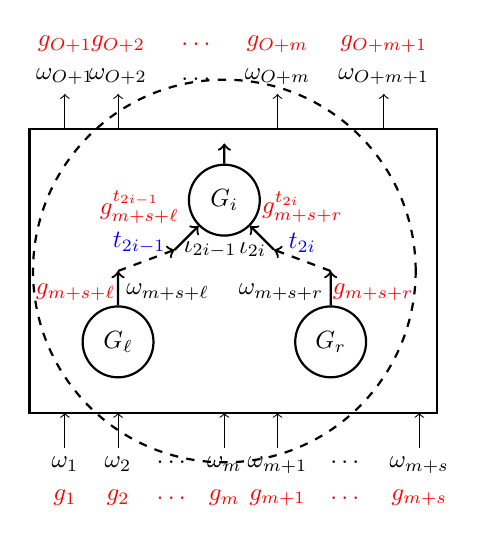
\begin{tikzpicture}[scale = 0.9, transform shape]
        \draw[thick] (0.25,0) rectangle (6,4);
        
       \node[circle, draw, thick, minimum size=1cm] (C) at (3, 3) {$G_i$};
        \node[circle, draw, thick, minimum size=1cm] (A) at (1.5, 1) {$G_\ell$};
        \node[circle, draw, thick, minimum size=1cm] (B) at (4.5, 1) {$G_r$};
            
        \draw[->, thick] (A.north) -- (1.5,2);
        \draw[->, thick] (B.north) -- (4.5,2);
        \draw[->, thick] (2.3,2.3) -- (C.south west);
        \draw[->, thick] (3.7,2.3) -- (C.south east);
        \draw[->, thick] (C.north) -- (3,3.8);

        \foreach \x/\y in {0.75/$\omega_1$, 1.5/$\omega_{2}$, 3/$\omega_{m}$, 3.75/$\omega_{m+1}$, 5.75/$\omega_{m+s}$} {
            \draw[<-] (\x, 0) -- ++(0, -0.5) node[below] {\y};
        }
        \node at (2.25,-0.7) {$\dots$};
        \node at (4.7,-0.7) {$\dots$};
        \foreach \x/\y in {0.75/$g_1$, 1.5/$g_{2}$, 3/$g_{m}$, 3.75/$g_{m+1}$, 5.75/$g_{m+s}$} {
            \node[red] at (\x,-1.2) {\y};
        }
        \node[red] at (2.25,-1.2) {$\dots$};
        \node[red] at (4.7,-1.2) {$\dots$};

        \foreach \x/\y in {0.75/$\omega_{O+1}$, 1.5/$\omega_{O+2}$, 3.75/$\omega_{O+m}$, 5.25/$\omega_{O+m+1}$} {
            \draw[->] (\x, 4) -- ++(0, 0.5) node[above] {\y};
        }    
        \node at (2.6,4.7) {$\dots$};
        \node[red] at (2.6,5.2) {$\dots$};
        \foreach \x/\y in {0.75/$g_{O+1}$, 1.5/$g_{O+2}$, 3.75/$g_{O+m}$, 5.25/$g_{O+m+1}$} {
            \node[red] at (\x, 5.2) {\y};
        }    

        \node at (2.2,1.7) {$\omega_{m+s+\ell}$};
        \node at (3.8,1.7) {$\omega_{m+s+r}$};
        \node[red] at (0.9,1.7) {$g_{m+s+\ell}$};
        \node[red] at (5.1,1.7) {$g_{m+s+r}$};
        \node[blue] at (1.8,2.4) {$t_{2i-1}$};
        \node[blue] at (4.1,2.4) {$t_{2i}$};
        \node at (2.8,2.3) {$\iota_{2i-1}$};
        \node at (3.4,2.3) {$\iota_{2i}$};
        \node[red] at (1.8,2.9) {$g_{m+s+\ell}^{t_{2i-1}}$};
        \node[red] at (4.1,2.9) {$g_{m+s+r}^{t_{2i}}$};
        \path[->]  (1.5,2) edge [thick,dashed]  (2.3,2.3)
                    (4.5,2) edge  [thick,dashed] (3.7,2.3);
        \draw[thick, dashed] (3,2) circle (2.7cm);
    \end{tikzpicture}
    \caption{Base labels: feed-in wires.}\label{fig:labellingingoingwires}
\end{figure}

In the open-specification step, the System knows the full circuit and can wire up the labels itself. When the circuit must also be hidden, the System no longer knows which feed-out wire connects to which feed-in wire. The challenge is to let the System prepare wire labels for garbling \emph{without} learning the circuit topology. We solve this by having the Monitor provide \emph{base labels}---random group elements associated with wires---from which the System derives the round-specific labels by exponentiation. The DDH assumption (\cref{assumption:DDH}) ensures that the exponentiated labels leak nothing about the wiring.

Since only the gate \emph{function} matters (and every gate is NAND), what must be hidden is the \emph{permutation} mapping feed-out wires to feed-in wires. The Monitor obfuscates this permutation using a cyclic group $\Gb$ of prime order~$q$ in which DDH holds.

\paragraph{Setup (round~0).}\label{protocol2}
The Monitor and System agree on the gate count~$c$, a security parameter~$n$, and the group~$\Gb$.

\begin{enumerate}
    \item \textbf{Feed-out base labels} (see \cref{fig:exponentsingoingwires}). The Monitor picks a random group element $g_i \xleftarrow{\$} \Gb$ for each non-output feed-out wire $\omega_i$ ($i \in \{1,\ldots,O\}$) and sends the list $[g_1,\ldots,g_O]$ to the System. The $m$~feedback output wires $\omega_{O+1},\ldots,\omega_{O+m}$ reuse the same base labels $g_1,\ldots,g_m$. The final output wire $\omega_{O+m+1}$ (the $\isbad$ bit) receives no base label during setup.
    \item \textbf{Feed-in base labels} (see \cref{fig:exponentsingoingwires,fig:labellingingoingwires}). For each feed-in wire $\iota_i$ ($i \in \{1,\ldots,I\}$), the Monitor draws a random exponent $t_i \xleftarrow{\$} \Zb_q$. Let $\pi(i) = j$ when feed-out wire~$\omega_j$ connects to feed-in wire~$\iota_i$. The Monitor computes $\ell_i = g_{\pi(i)}^{t_i}$ and sends the list $[\ell_1,\ldots,\ell_I]$ to the System.
    \item \textbf{Oblivious transfer.} Exactly as in the open-specification step: the System sends random label pairs for the $m$~state wires, and the Monitor uses OT to obtain the labels corresponding to $\mu[1]$.
\end{enumerate}

The System now holds three base labels per gate (two feed-in, one feed-out) but cannot tell which feed-out wire each feed-in label was derived from: by the DDH assumption (\cref{lemma:DDHprop}), the tuple $(\ell_1,\ldots,\ell_I)$ is indistinguishable from $I$~uniformly random group elements, regardless of the permutation~$\pi$.

\paragraph{Round~$r$ ($r \geq 1$).}
The System holds $\sigma[r]$ and proceeds as follows.

\begin{enumerate}
    \item \textbf{Choose round exponents.} In round~$1$ the System picks distinct $\alpha^0[1],\alpha^1[1] \xleftarrow{\$} \Zb_q$. In subsequent rounds, it reuses the output exponents from the previous round: $\alpha^b[r] \gets \beta^b[r{-}1]$.
    \item \textbf{Derive feed-out labels.} For each non-output feed-out wire $\omega_j$ ($j \in \{1,\ldots,O\}$):
    $w_j^b[r] = g_j^{\alpha^b[r]}$.
    The System also draws fresh $\beta^0[r],\beta^1[r] \xleftarrow{\$} \Zb_q$ and sets the feedback-output labels $w_{O+j}^b[r] = g_j^{\beta^b[r]}$ for $j \in \{1,\ldots,m\}$. For the $\isbad$ output wire $\omega_{O+m+1}$, it picks $w_{O+m+1}^0[r],w_{O+m+1}^1[r] \xleftarrow{\$} \Gb$ (random group elements, not derived from a base label).
    \item \textbf{Derive feed-in labels.} For each feed-in wire $\iota_i$: $u_i^b[r] = \ell_i^{\alpha^b[r]}$.
    \item \textbf{Garble and send.} Same as in the open-specification step: garble every gate $G_j$ using the feed-in labels $(u_{2j-1}^b[r], u_{2j}^b[r])$ and feed-out label $w_{m+s+j}^b[r]$, and send all garbled gates, the System's input labels, and both flag labels.
    \item \textbf{Evaluate.} The Monitor ungarbles bottom-up. After obtaining the feed-out label $w_{m+s+j}^{b^*}[r] = g_{m+s+j}^{\alpha^{b^*}[r]}$ from gate~$G_j$, the Monitor raises it to the exponent~$t_i$ of the downstream feed-in wire~$\iota_i$ to recover the feed-in label: $(g_{m+s+j}^{\alpha^{b^*}[r]})^{t_i} = (g_{m+s+j}^{t_i})^{\alpha^{b^*}[r]} = \ell_i^{\alpha^{b^*}[r]} = u_i^{b^*}[r]$. In other words, the Monitor can propagate labels through the circuit by exponentiating, without the System ever revealing the wiring.
\end{enumerate}

\noindent Because $\alpha^b[r{+}1] = \beta^b[r]$ and the feedback base labels coincide with the state-input base labels ($g_1,\ldots,g_m$), the label-reuse mechanism from the open-specification step carries over: the Monitor's state-output labels from round~$r$ serve directly as state-input labels for round~$r{+}1$, preserving reactivity.

Both message sizes and computation time are linear in $c{+}s{+}m$ (assuming the security parameter is a constant).

\begin{restatable}{theorem}{Protocoltwosecure}\label{thm:Protocol2secure}
    Under CPA-secure encryption, the DDH assumption on $\Gb$, and semi-honest oblivious transfer, the hidden-specification step is a correct and secure monitoring protocol with specification hiding for any polynomial number of rounds.
\end{restatable}

The proof constructs intermediate indistinguishable transcripts by progressively replacing elements with random group elements. A key ingredient is a corollary of \cref{lemma:DDHprop} from Naor and Reingold~\cite{NR04}; the same lemma is used in the work of Liu, Wang, and Yu~\cite[Lemma~3]{LWY22}. The full proof appears in \cref{app:proofs}.
